\documentclass[12pt,a4paper]{article}

\usepackage[left=0.8in, right=0.8in, top=0.5in, bottom=0.8in]{geometry}
\usepackage{caption}
\usepackage{graphicx}
\usepackage{subcaption}
\usepackage{amsmath}
\usepackage{algpseudocode}
\usepackage{algorithm}
\usepackage{wrapfig}

%\usepackage{mwe}


%opening
\title{\vspace{-1.5cm}\huge{Structural Reconstruction of a Ruined Building}\\ \vspace{0.5cm}\Large{Project Final Report}\\\vspace{0.4cm}\large{CS5240 - Theoretical Foundations in Multimedia}\\
    \large{Project Group : P-03}}


\date{}


\begin{document}
    
    \maketitle
    \vspace{-2cm}
    \begin{table}[h]
        \centering
        \begin{tabular}{cc}
            \textbf{\large{Anshul Aggarwal}} & \textbf{\large{Gogula Krishnan Saravanan}}      \vspace{0.2cm}\\
            A0191501R                & A0191385X                               \vspace{0.5cm}\\
            \textbf{\large{Manasa Kashyap}}  & \textbf{\large{Meenakshi Sundaram Viswanathan}} \vspace{0.2cm}\\
            A0178462W                & A0191324L                              
        \end{tabular}
    \end{table}
    
    %\begin{abstract}
    
    %\end{abstract}
    
    \section{Introduction}
    
    Ruined buildings, or simply ruins, are the remains of the man-made buildings. Over the passage of time, due to various reasons such as natural disaster, deliberate acts of destruction, or simply weathering and lack of maintenance, only parts of the original building remain today.
    
    \begin{wrapfigure}{R}{0.38\textwidth}
        \centering
        \captionsetup{justification=centering}
        
        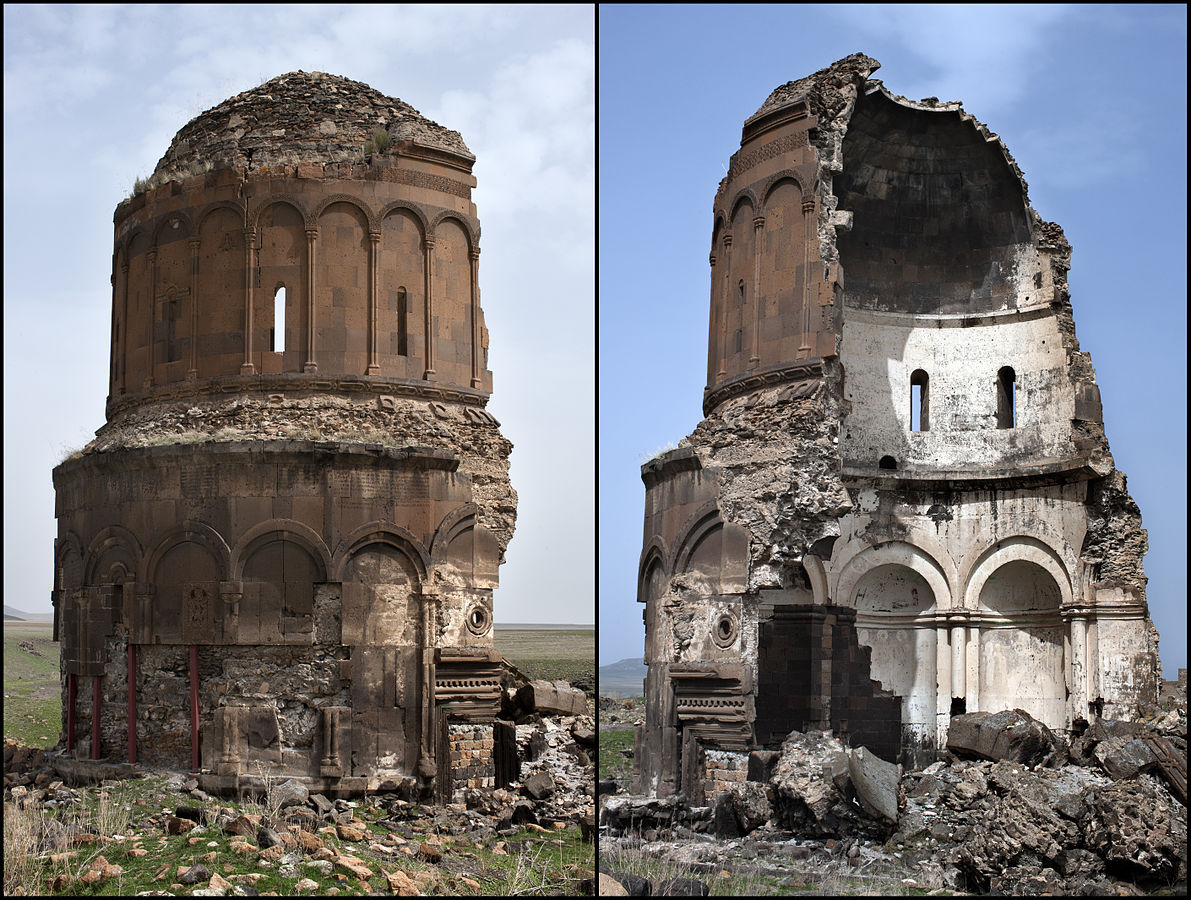
\includegraphics[width=0.35\textwidth]{ruins.jpg}
        
        \caption{The Church of the Holy Redeemer -- Ani, Turkey}
        \label{fig:ruins}
    \end{wrapfigure}
    
    There are various scenarios where reconstructed models of these ruined buildings may be useful. Archaeologists and historians refer to ruins of ancient buildings (like the one shown in Fig. \ref{fig:ruins}) to study civilizations, their style of architecture, and their culture. A fully reconstructed model may help them study the structure better. Other than that, engineers need to fix damages to buildings caused by natural disasters or explosions, and such a reconstructed model will help them plan out repairs.
    
    Our work here aims to efficiently employ data fitting/model fitting techniques to reconstruct the defining structures of any dilapidated building, so as to achieve a structure that closely resembles the original structural design of the building under consideration.
    
    
    
    \section{Variables and Relationships}
    
    A 3-dimensional point cloud of the existing structure will act as the input to our problem. These points may have been captured using 3D Laser Scanning, or obtained by any other means.
    
    We try to reconstruct surfaces from these points by defining relationships, or functions over the 3D space which are satisfied by the input points, such that they best represent the original shape of the building. These surfaces may represent walls, ceilings, floors, or any other surfaces.
    
    \section{Problem Definition}
    
    \subsection{Objective}
    
    Given a point cloud representation of a ruined building, obtain surface functions of the building to recreate a model of the building that could best represent it before it was damaged.
    
    \subsection{Input}
    
    \begin{itemize}
        \itemsep0em 
        \item $n$ data points capturing external structure of ruined building with 3D coordinates $p_i = (x_i, y_i, z_i)$, $i = 1,\dots,n$; $S=\left\{p_{1},p_{2},\dots,p_{n}\right\}$
        \item Number of surfaces, $k$, and their rough centroids $c_j, j=1, \dots, k$.
    \end{itemize}
    
    \subsection{Outputs}
    
    \begin{itemize}
        \itemsep0em 

        \item $k$ segmented sets of points $S_j \subset S, j=1,\dots,k$, with points belonging to the same set considered to be a part of the same surface.
        \item Boundary limits of $S_j$ given by polyhedron $B_j$.
        \item $k$ linear or non-linear surface functions $f_j(p), j=1,\dots,k$
        
        
    \end{itemize}
    
    \subsection{Constraints}
    
    \begin{itemize}
        \item For all points $p_i \in S_j$, the spatial error $E_j$ is minimized for each surface $f_j, j=1,\dots,k$, by the following optimization objective
        \begin{equation}
        \textrm{Minimize } E_j = \sum_{p_i \in S_j} {||f_j(p_i) - p_i ||^2} %Standard minimization notation, and makes single glance read easier to understand%
        \end{equation}
    \end{itemize}
    
    \section{Problem Solving Approach}
    
    The problem can be broadly divided into several sub-problems, that handle different stages in solving the complete problem. These are:
    
    \begin{enumerate}
        \item \textbf{Point Cloud Segmentation:} Divide point-cloud into sets of points belonging to same surface.
        \item \textbf{Surface Fitting:} Perform robust piecewise polynomial surface fitting to each point set.
        \item \textbf{Defining Surface Bounds and Reconstruction:} Find the bounds of the surfaces, and then generate dense point cloud of the reconstructed structure.
    \end{enumerate}
    
    Each of the above sub-problems has been described in detail as under.
    
    \subsection{Point Cloud Segmentation}
    
    This step is used to divide points in the point cloud into point sets which in turn will form independent surfaces that will be required to construct a model of the building, with the given data. Through this process, we identify different sets of points such that points belonging to the same set are used to fit a single surface.
    
    We simply use a \textbf{modified region growing algorithm} for this process. The algorithm iteratively accumulates the points that can lie on a simple surface, into the same set until all points are covered. This is achieved by comparing the angles between the estimated-point-normals. If the angles are greater than a threshold value, the points cannot be said to form a part of the same surface, and thus must belong to separate surface sets.
    
    Consider an example point cloud as shown in Fig. \ref{fig:pcloud}. Point sets for this point cloud have been identified, with unique sets marked by different colours in Fig. \ref{fig:psets}.
    

    \subsubsection{Inputs}
    \begin{itemize}
        \itemsep0em 
        \item Point cloud of a ruined building, $p_i \in S$
        \item Number of surfaces, $k$.
        \item Approximate centroids $c_{j}, j=1,\dots,n$
        \item Normal-angle difference threshold $\theta$
        \item Neighbourhood points discovery function $N$.
        \item Estimated-point-normal (EPN) calculation function $T$.
    \end{itemize}
    
    \subsubsection{Outputs}
    \begin{itemize}
        \itemsep0em 
        \item Segmented sets of points $S_j \subset S, j=1,\dots,k$, with points belonging to the same set considered to be a part of the same surface.
    \end{itemize}

    \subsubsection{Algorithm}
    \begin{algorithm}[H]
        \caption{Modified Region-growing Point Cloud Segmentation}
        \begin{algorithmic}
            \ForAll {centroids $c_j$}
            \State Initialize seeds set $Sd = \{c_j\}$, Surface set $S_j = \emptyset$
            \ForAll {Seed point $r$ in $Sd$}
                \ForAll {Neighbourhood point $q$ in set of points obtained from $N(r)$}
                \If {angle between EPNs of seed, current point $|T(q) - T(r)| < \theta$}
                \State Add $q$ to $Sd$ and $S_j$
                \EndIf
                
            \EndFor
            \State Remove seed point $r$ from $Sd$
            \EndFor
            \EndFor
        \end{algorithmic}
    \end{algorithm}
    
    \begin{figure*}
        \centering
        \begin{subfigure}[b]{0.23\textwidth}
            \centering
            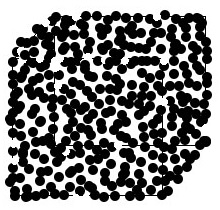
\includegraphics[width=\textwidth]{point_cloud.jpg}
            \caption{Point Cloud}
             \label{fig:pcloud}
        \end{subfigure}%
        \quad \quad
        \begin{subfigure}[b]{0.23\textwidth}
            \centering
            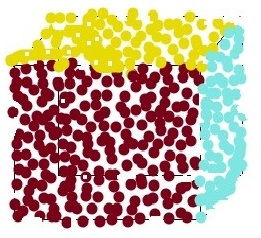
\includegraphics[width=\textwidth]{cube1.jpg}
            \caption{Segmented Point Sets}
            \label{fig:psets}
        \end{subfigure}%
        \quad \quad
        \begin{subfigure}[b]{0.23\textwidth}
            \centering
            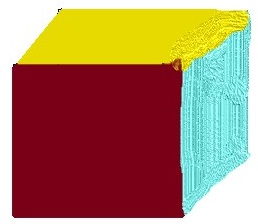
\includegraphics[width=\textwidth]{planes.jpg}
            \caption{Bounded Surface Fits}
            \label{fig:planes}
        \end{subfigure}%
        
        \caption{Point-cloud segmentation and surface fitting}
    \end{figure*}
    
    
    \subsection{Surface Fitting}
    
    Once the sets that belong to the same surface are obtained, a robust piecewise polynomial surface is fit over the points in each set. Considering a general equation of a polynomial surface, we can use least squares error minimization as an objective function to obtain the parameters of the polynomial surface which best fits the points in the surface set.
    
    For this problem, if we simply use quadratic surfaces for data fitting using least squares error minimization algorithm, this may not be sufficient in case of complex curved surfaces, which may not be modelled well using a small number of surface functions. To address this, we use a piecewise quadratic surface fitting system, where we use multiple smaller surfaces per building feature to fit the point cloud. We divide the surface point-sets into smaller sub-surface sets which consider points in small neighbourhoods, which are then used with a piecewise surface fitting algorithm as described below.
    
    \subsubsection{Inputs}
    \begin{itemize}
        \itemsep0em
        \item $k$ segmented sets of points $S_j \subset S, j=1,\dots,k$, with points belonging to the same set considered to be a part of the same surface.
        \item Neighbourhood points discovery function $N$.
        \item Nearest neighbouring cluster function, $L$.
    \end{itemize}
    
    \subsubsection{Outputs}
    Parameters of surface functions $f_j, j=1,\dots,k$
    
    \[
    f_{j}(p)=\left\{\begin{array}{ll}{f_{j1}(p),}&{\text{if } L(p)=S_{j1}}\\{f_{j2}(p),}&{\text{if }L(p)=S_{j2}}\\{}&{\vdots}\\{f_{jm}(p),}&{\text{if }L(p)=S_{jm}}\end{array}\right.
    \]
    
    \noindent where $S_{jq} \subset S_{j}, q=1,\dots,m$ and $\bigcup\limits_{q=1}^{m} {S_{jq}} = S_j$.\\
    \noindent $f_{jq},q=1,\dots,m$ are quadratic 3D functions with parameter $\textbf{A}_{jq}$ satisfying the following equation
    
    \begin{equation}
    \begin{split}
    f_{jq}(p) & =
    \left[\begin{array}{ccccccc}{x^{2}}&{y^{2}}&{z^{2}}&{xy}&{yz}&{xz}&{1}\end{array}\right]
    \left[\begin{array}{ccc}a_{200}&b_{200}&c_{200}\\a_{020}&b_{020}&c_{020}\\a_{002}&b_{002}&c_{002}\\a_{110}& b_{110}& c_{110}\\a_{011}&b_{010}&c_{011}\\a_{101}&b_{101}&c_{101}\\a_{000}&b_{000}&c_{000}\end{array}\right]\\
    & = \left[\begin{array}{ccccccc}{x^{2}}&{y^{2}}&{z^{2}}&{xy}&{yz}&{xz}&{1}\end{array}\right] \textbf{A}_{jq}
    \end{split}
    \end{equation}
    
    \noindent For the subset  $S_{jq}, q=1,\dots,m$ having $r$ points, we get
    
    \begin{equation}
    \left[\begin{array}{ccccccc}{x_{1}^{2}}&{y_{1}^{2}}&{z_{1}^{2}}&{x_{1}y_{1}}&{y_{1}z_{1}}&{x_{1}z_{1}}&{1}\\{}&{}&{}&{\vdots}&{}&{}&{}\\{x_{r}^{2}}&{y_{r}^{2}}&{z_{r}^{2}}&{x_{r}y_{r}}&{y_{r}z_{r}}&{x_{r}z_{r}}&{1}\end{array}\right]A_{jq}=\left[\begin{array}{ccc}{x_{1}}&{y_{1}}&{z_{1}}\\{}&{\vdots}&{}\\{x_{r}}&{y_{r}}&{z_{r}}\end{array}\right]
    \end{equation}
    
    \begin{equation}
    \textbf{D} \textbf{A}_{jq}=\textbf{U}
    \end{equation}
    
    \begin{equation}\label{fittingeq}
    \textbf{A}_{jq}=\left(\textbf{D}^\top \textbf{D}\right)^{-1}\textbf{D}^\top \textbf{U}
    \end{equation}
    
    \subsubsection{Algorithm}
    \begin{algorithm}[H]
        \caption{Piecewise Robust Polynomial Surface Fitting}
        \begin{algorithmic}
            \ForAll{surface sets $S_j$}
            \State Initialize available points list $\textbf{T} = S_j$
            \Repeat
            \State Initialize $p$ with a point in $T$
            \State Initialize $S_{jq}$ with neighbouring set of points from $N(p)$
            \State Remove points in set $S_{jq}$ from $T$
            \State Trim $S_{jq}$ to remove outliers
            \State Use $S_{jq}$ to solve for parameters $\textbf{A}_{jq}$ of function $f_{jq}$ using Eq. \ref{fittingeq}.
            \Until {$\textbf{T}$ is empty} 
            \EndFor
        \end{algorithmic}
    \end{algorithm}
    
    
    
    \subsection{Defining Surface Bounds and Reconstruction}
    
    Given all the polynomial surfaces obtained in the data fitting step, we need to define the surface boundaries by finding bounds for obtained point sets. This gives us enough information to reconstruct the structure. A bounded surface fit example is shown in Fig. \ref{fig:planes}. Then, we generate a dense point cloud of the reconstructed structure, which can be used for further applications.   
    
%    In rare cases, it is possible that one or more sides of the surfaces may not end up being constrained, which means the surface in consideration remains an infinite surface. This may be due to extensive damage to the building that may have led to complete loss of defining features, and in some cases information of a dimension of the building. Or, in other cases, a surface function may be influenced significantly by some noise in the data, that makes the surface extend way beyond the actual building design. This can be tackled by considering a minimum point density for a region of surface to be valid. If the point density falls below a certain threshold for some region of the surface (zero in case of missing feature information), the corresponding region of the surface will not be considered, and the surface will be bounded to the region where the point density is above the density threshold.
    
    
    \subsubsection{Inputs}
    \begin{itemize}
        \itemsep0em 
        \item $k$ segmented sets of points $S_j \subset S, j=1,\dots,k$, with points belonging to the same set considered to be a part of the same surface.
        \item Surface functions $f_j, j=1,\dots,k$
        \item Alpha shape function, $G$
    \end{itemize}
    
    
    \subsubsection{Outputs}
    \begin{itemize}
        \item Point cloud $S^\prime$ representing the reconstructed building.
    \end{itemize}
    
    \subsubsection{Algorithm}
    \begin{algorithm}[H]
        \caption{Reconstruction}
        \begin{algorithmic}
            \State Initialize reconstructed building's point cloud $S^\prime = \emptyset$
            \ForAll {Surface sets $S_j$}
            \State Initialize polyhedron $B_j = G(S_j)$
            \ForAll{points $p$ within $B_j$}
            \State Add  $f_j(p)$ to $S^\prime$
            \EndFor
            \EndFor
        \end{algorithmic}
    \end{algorithm}


    \subsection{Compiling the process}
    
    Overall, the whole algorithm can be described as follows.
    
    \begin{algorithm}[H]
        \caption{Compiled algorithm}
        \begin{algorithmic}
            \State 1. Grow surface sets using \textbf{modified region-growing point cloud segmentation}.
            \State 2. Fit surfaces on the surface sets using \textbf{robust piecewise polynomial surface fitting}.
            \State 3. Define surface bounds for each obtained surface and \textbf{reconstruct} a dense point cloud.
        \end{algorithmic}
    \end{algorithm}
    
    
    \section{Observations \& Issues}\label{issues}
    
    There may be instances where some information about the building structure is completely lost. This lost information cannot be regained. For example, if an asymmetric or non-uniform corner of a building is completely lost, the reconstruction may not be able to accurately reflect the original building, as there is no information to define the asymmetry.
    
    An extension of this problem is when information about a dimension of the building is lost. This may lead to multiple output reconstructed models based on different guesses for the missing dimension.
    
    \section{Problem Instance and Expected Results}
    
        \begin{wrapfigure}{R}{0.65\textwidth}
        \centering
        \begin{subfigure}[b]{0.3\textwidth}
            \centering
            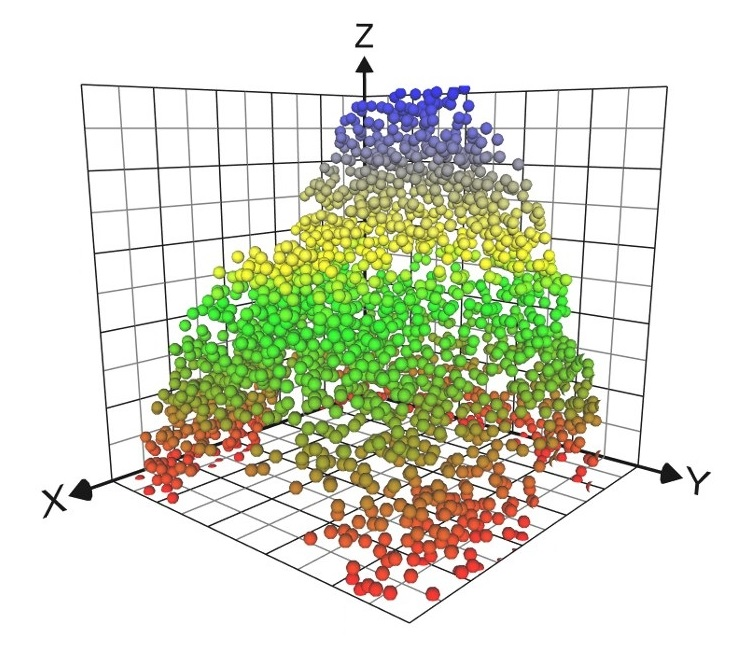
\includegraphics[width=\textwidth]{scatter1.jpg}
            \caption[]{{\small Point cloud representation of a ruined building}}    
            \label{fig:scatter}
        \end{subfigure}
        \quad
        \begin{subfigure}[b]{0.3\textwidth}  
            \centering 
            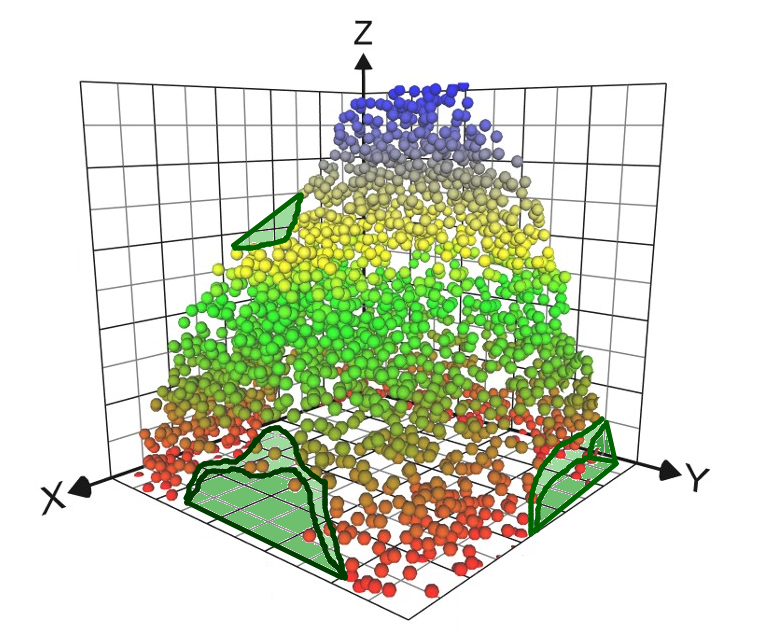
\includegraphics[width=\textwidth]{missing2.png}
            \caption[]{{\small Missing or damaged parts of the building}}    
            \label{fig:missing}
        \end{subfigure}
        \vskip\baselineskip
        \begin{subfigure}[b]{0.3\textwidth}   
            \centering 
            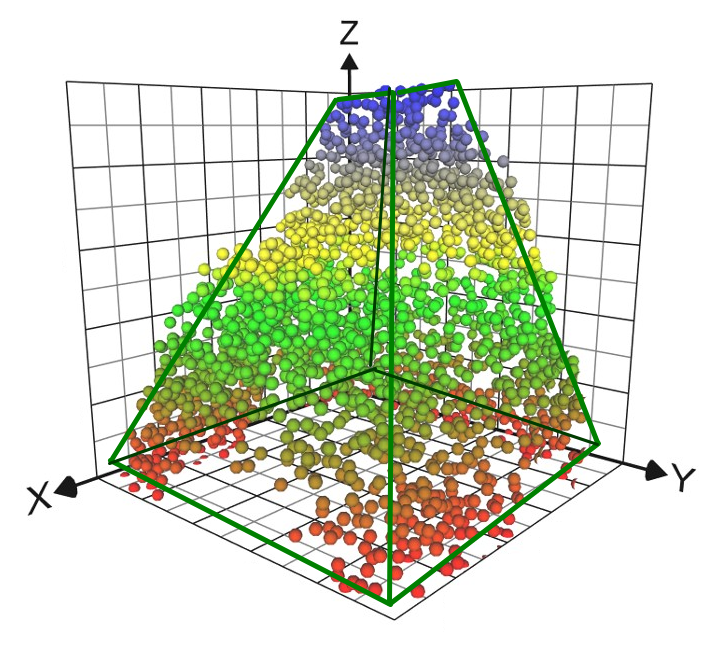
\includegraphics[width=\textwidth]{reconstruction.png}
            \caption[]{{\small Reconstruction scenario 1 - levelling of the planes at the top}}    
            \label{fig:rec1}
        \end{subfigure}
        \quad
        \begin{subfigure}[b]{0.3\textwidth}   
            \centering 
            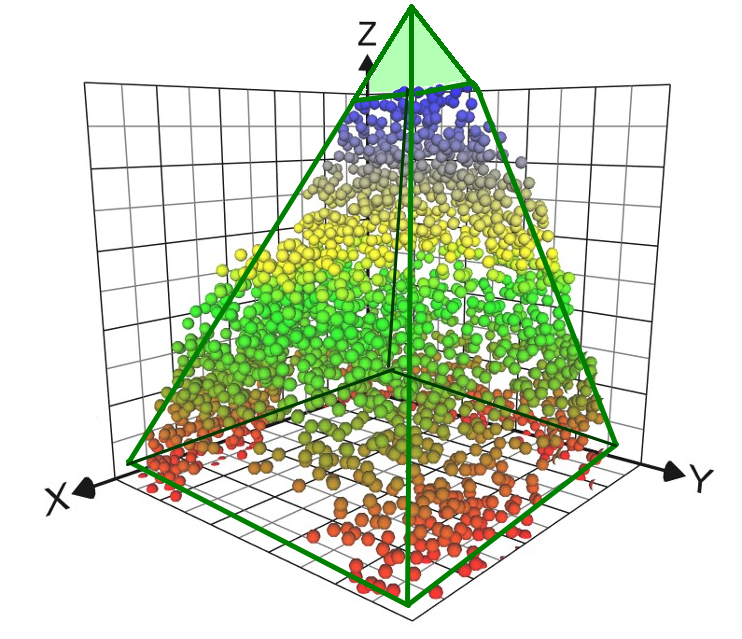
\includegraphics[width=\textwidth]{reconstruction2.png}
            \caption[] {{\small Reconstruction scenario 2 - extending planes to a point intersection}}    
            \label{fig:rec2}
        \end{subfigure}
        \caption[]{\small An example problem and solution} 
        \label{fig:example}
    \end{wrapfigure}
    
    Let us consider an example. Fig. \ref{fig:scatter} shows the point cloud of a dilapidated, ruined building. To an observer, there may be a few obvious missing parts of the building, or regions in the 3D space where the point density is high in the neighbourhood, while zero in the given region. This is represented in Fig. \ref{fig:missing}.
    
    It is however difficult to represent the regions with zero point density in computational terms. We therefore use data fitting to obtain surfaces that best fit the given data points, we can get the missing or damaged portions of the building. There may however be multiple possible reconstructions, as discussed in section \ref{issues} above. Considering two different reconstruction scenarios, we may get two distinct models, as shown in Fig. \ref{fig:rec1}, \ref{fig:rec2}. These reconstructed models however only differ mostly in the intersection based bounds for the fitted surfaces, and not the surfaces themselves.
    
    In this project however, we do not \textit{guesstimate} unknown features to avoid possible ambiguity. So, the case shown in Fig. \ref{fig:rec2} will not be generated.
    
    %and considering these surfaces shall intersect to define boundaries, 
    
    
\end{document}
